\documentclass[asp1.tex]{subfiles}
\begin{document}

\section{ITS Hä}

\subsection{Strukturierte Verkabelung}

Eine strukturierte Verkabelung ist ein einheitlicher Aufbauplan für eine Netzwerkinfrastruktur, auf der unterschiedliche Dienste (Sprache oder Daten) übertragen werden.

Es basiert auf einer allgemein gültigen Verkabelungsstruktur, die auch die Anforderungen mehrerer Jahrzehnte berücksichtigt, Reserven enthält, flexibel erweiterbar ist und unabhängig von der Anwendung genutzt werden kann.

Durch diesen Plan sollen Fehlinstallationen vermieden und die Installation neuer Netzwerkkomponenten erleichtert werden.

\break

Es wird in 3 Bereiche unterschieden:
\begin{itemize}
    \item Geländeverkabelung (Prim\"ar)
        \begin{itemize}
            \item große Distanz
            \item große \"Ubertragungsraten
            \item meist Glasfaser
        \end{itemize}
    \item Gebäudeverkabelung (Sekund\"ar)
        \begin{itemize}
            \item kurze bis mittlere Distanz
            \item Kabel vom Geb\"audeverteiler zu Etagenverteilern
            \item Glasfaser oder Kupfer
            \item max 500m
        \end{itemize}
    \item Etagenverkabelung (Terti\"ar)
        \begin{itemize}
            \item kurze Distanz
            \item Twisted-Pair-Kabel
            \item max 90m
            \item M\"undung in Anschlussdosen
        \end{itemize}
\end{itemize}
\begin{figure}[H]
\begin{center}
  \includegraphics[height=6cm]{struk.png}
  \end{center}
  \caption{Strukturierte Verkabelung}
  \label{fig:Strukturierte Verkabelung}
\end{figure}
\break

\subsection{IPv4}

Eine IPv4-Adresse folgt dem Schema:

\(<0-255>.<0-255>.<0-255>.<0-255>\)

Beispiel: 192.168.0.1

Es stehen 32 Bit zur Verfügung \textrightarrow\space \(2^{32}\) \textrightarrow\space ca. 4 Mrd. IPv4 Adressen

\textbf{Spezielle IPv4 Netze:}
\begin{itemize}
    \item 127.x.x.x /8 \textrightarrow\space Loopback/Localhost (gilt für gesamtes 127er Netz)
    \item private IPv4 Netze:
        \begin{itemize}
            \item 10.0.0.0 /8
            \item 172.16.0.0 /12
            \item 192.168.0.0 /16
        \end{itemize}
\end{itemize}

\subsubsection{IPv4 Subnetting}

Es wird zwischen zwei Arten des Subnettings unterschieden:
\begin{itemize}
    \item \textbf{Symmetrisch}: Es entstehen n gleich große Subnetze
    \item \textbf{Asymmetrisch}: Es entstehen unterschiedlich große Subnetze
\end{itemize}

\textbf{Symmetrisches Subnetting}

Vorgehensweise mit Beispiel:

Ausgangsnetz: 10.0.0.0 /8\\
Ziel: Netz in drei Subnetze aufteilen

\textbf{1. Schritt:} Anzahl der zusätzlichen Netzbits bestimmen:\\
Da das Netz in drei Subnetze zerlegt werden soll, benötigen wir zwei zusätzliche Netzbits.\\
Begründung: Die nächst höhere Zweierpotenz ist 4 \textrightarrow\space \(2^\textbf{2} = 4\) \textrightarrow\space Zwei zusätzliche Netzbits

\textbf{2. Schritt:} Subnetzmaske / Slash-Darstellung anpassen\\
Aus 10.0.0.0 /8 wird nun 10.0.0.0 /10

\textbf{3. Schritt:} Netze bilden\\
Für die NetzID der Netze werden alle verfügbaren Hostbits auf 0 gesetzt. Um die jeweiligen Subnetze zu bilden, müssen nur die hinzugefügten Netzbits hochgezählt werden (00 \textrightarrow\space 01 \textrightarrow\space 10). Das vierte so entstehende Subnetz kann für diese Aufgabe ignoriert werden, da nur nach drei Netzen gefragt ist.

Erstes Subnetz: \textbf{10.0.0.0 /10}\\
Zweites Subnetz: \textbf{10.64.0.0 /10}\\
Drittes Subnetz: \textbf{10.128.0.0 /10}

Genauere Darstellung \href{https://jodies.de/ipcalc?host=10.0.0.0&mask1=8&mask2=10}{hier}.

\break

\textbf{Asymmetrisches Subnetting}

Asymmetrisches Subnetting wird genutzt, um Subnetze für eine bestimmte Anzahl an Clients zu erstellen.

Vorgehensweise mit Beispiel:

Ausgangsnetz: 10.0.0.0 /8\\
Ziel: 2 * 500 Hosts \textbf{+} 3 * 16 Hosts

\textbf{Immer mit dem größten Netz anfangen!}

\textbf{1. Schritt:} Anzahl der Netzbits bestimmen:\\
Für Netze mit 500 Hosts: 9 Hostbits (\(2^\textbf{9} = 512\)) \textrightarrow\space \(32-9 = 23\) Netzbits.

Für Netze mit 16 Hosts: 5 Hostbits (\(2^\textbf{5} = 32\) \textbf{(Es werden 32 IPs benötigt, da 16 IPs nicht für 16 Hosts reichen - Broadcast und Netz-ID können nicht vergeben werden!)})\textrightarrow\space \(32-5 = 27\) Netzbits.

\textbf{Schritt 2:} Subnetze bilden:\\
Für die Bildung des ersten Subnetzes, muss nur die Subnetzmaske/Slash-Notation angepasst werden:\\
1. Subnetz: 10.0.0.0 /23; Broadcast: 10.0.1.255

Um das zweite Subnetz zu bilden, wird die Broadcast IP des vorherigen Netzes um eins erhöht. Dies ergibt die Netz-ID des zweiten Netzes:\\
2. Subnetz: 10.0.2.0 /23; Broadcast: 10.0.3.255

Das gleiche Prinzip wir für das zweite Netz kann nun fortgeführt werden.
3. Subnetz: 10.0.4.0 /23; Broadcast: 10.0.5.255

\textit{Wenn nach einer hohen Anzahl von Netzen gefragt ist, kann nach einem Muster in den Netz-IDs gesucht werden, um den Prozess zu beschleunigen. In diesem Beispiel erhöht sich der 3. Block der IP immer um 2.}

Für das vierte Subnetz (das erste mit der neuen Hostanzahl), kann der gleiche Prozess für die Netz-ID angewendet werden wie zuvor (Broadcast des letzten Netzes + 1 = Netz-ID des neuen Netzes). Allerdings muss hier darauf geachtet werden, dass die Subnetzmaske/Slash-Notation angepasst wird!\\
4. Subnetz: 10.0.6.0 /27; Broadcast: 10.0.6.31

Für das fünfte Subnetz wird wieder die Broadcast IP des vorherigen Netzes um eins erhöht\\
5. Subnetz: 10.0.6.32 /27


\break
\subsection{IPv6}

Eine IPv6 Adresse folgt dem Schema:

\textless0-ffff\textgreater:\textless0-ffff\textgreater:\textless0-ffff\textgreater:\textless0-ffff\textgreater:\textless0-ffff\textgreater:\textless0-ffff\textgreater:\textless0-ffff\textgreater:\textless0-ffff\textgreater

Beispiel: fe80:0000:0000:0000:7d45:0db9:c2c2:ab7b

Es stehen 128 Bit zur Verfügung \textrightarrow\space \(2^{128}\) \textrightarrow\space ca. \(3.4 * 10^{38}\) IPv6 Adressen (340 Sextillionen).

Die IPv6 Adresse wird in 8 Blöcke mit jeweils 16 Bit unterteilt, die durch ein ':' getrennt werden.\\
Innerhalb eines Blocks dürfen \textbf{führende} Nullen weggelassen werden.\\
Eine Folge von 0er-Blöcken darf \textbf{einmalig} durch '::' ersetzt werden.

Die Beispiel Adresse lässt sich so wie folgt kürzen:\\
fe80::7d45:db9:c2c2:ab7b

Die ersten vier Blöcke bilden den Prefix (Netzbits) und die letzten 4 den Identifier (Hostbits) der IPv6 Adresse.

\subsubsection{Der Identifier}
Der Identifier wird nach EUI64 aus der MAC Adresse des Gerätes gebildet und kennzeichnet den Host. Dabei wird in die Mitte der MAC Adresse 'fffe' eingeschoben, um auf die korrekte Anzahl an Bits zu kommen. Abschließend wird das siebte Bit invertiert.\\
Beispiel:

MAC: 48:17:BC:12:46:98

fffe einflicken: 4817:bcff:fe12:4698

Siebtes Bit invertieren: 4a17:bcff:fe12:4698

Da Nutzer mit IPv6 Adressen die durch dieses Verfahren gebildet wurden leicht im Internet getrackt werden können (IP lässt sich in MAC Adresse umwandeln), gibt es die \textbf{privacy extensions}.\\
Sie randomisieren den Identifier um das Tracking zu verhindern.

\subsubsection{Das Prefix}

Das Prefix kennzeichnet das Netz/Subnetz. Die von IPv4 bekannte Subnetzmaske fällt bei IPv6 komplett weg. Um dennoch eine Unterteilung der Netze zu ermöglichen, wird die Prefixlänge nach der IPv6 Adresse mit einem '/' angegeben. /56 beispielsweise meint, dass der Prefix die ersten 56 Bit der Adresse sind. Die Bits 57 bis 64 (die restlichen des gesamten Prefix) können zum Subnetten verwendet werden.

\textbf{Besondere Prefixe:}
\begin{itemize}
    \item fe80:: /10 \textrightarrow\space Link-Local-Address (entspricht IPv4 APIPA)\\
        \begin{itemize}
            \item Die restlichen Bits des Prefixes sind zu nullen!
            \item Wird genutzt um nach dem hochfahren des Geräts eine im LAN gültige IPv6 Adresse zu haben, mit der sich das Gerät den Prefix des Netzes suchen kann.
        \end{itemize}
    \item 2000:: /3 \textrightarrow\space Global-Address (= Öffentliche IP) \textbf{da '/3' ist auch 3000:: eine globale IPv6}
        \begin{itemize}
            \item Bits 4 bis 40 werden zur Länder- und Providerkennung genutzt.
            \item Bits 41 bis 64 können zum Subnetting genutzt werden
        \end{itemize}
    \item FC00:: /7 \textrightarrow\space Unique-Local-Address (Eigentlich immer \textbf{FD00:: /8}, da 8. Bit (l-Bit) so von IANA festgelegt)
       \begin{itemize}
           \item Bits 9 bis 48 können frei vom Admin vergeben werden (Um Kollisionen beim zusammenfügen von Netzen zu vermeiden sollte diese zufällig gewählt werden)
           \item Bits 41 bis 64 können zum Subnetting genutzt werden
       \end{itemize}
\end{itemize}

Die oben genannten Prefixe gehören alle zu \textbf{Unicast} Adressen:
\begin{itemize}
    \item Unicast: Einer an Einen
    \item Broadcast: Einer an Alle \textbf{(Gibt es nicht in IPv6)}
    \item Multicast: Einer an Viele (FF00:: /8)
\end{itemize}

\textbf{Besondere IPv6 Adressen:}
\begin{itemize}
    \item :: \textrightarrow\space Unspecified Address, wird direkt nach dem Start des Geräts als IPv6 Adresse genutzt
    \item ::1 \textrightarrow\space Loopback Address
\end{itemize}

\subsubsection{IPv6 Subnetting}

Vorgehensweise mimt Beispiel:

Prefix: fd00:1:2:: /52 \\
Ziel: 16 Subnetze

\textbf{1. Schritt:} Anzahl der zusätzlichen Netzbits bestimmen:\\
Für 16 Subnetze werden 4 zusätzliche Netzbits benötigt.\\
Begründung: Die nächst höhere Zweierpotenz ist 16 \textrightarrow\space \(2^\textbf{4} = 16\) \textrightarrow\space Vier zusätzliche Netzbits

\textbf{2. Schritt:} Zusätzliche Bits zur Slash-Notation hinzufügen:\\
fd00:1:2:: /56

\textbf{3. Schritt:} Subnetze bilden:\\
Um die Prefixe der Subnetze zu bilden, müssen nur die  hinzugefügten Netzbits hochgezählt werden. (0000\textrightarrow\space0001\textrightarrow\space0010\textrightarrow\space...).

1. Subnetz: fd00:1:2:: /56\\
2. Subnetz: fd00:1:2:100:: /56\\
3. Subnetz: fd00:1:2:200:: /56\\
.\\
.\\
.\\
16. Subnetz: fd00:1:2:F00 /56\\

Genauere Darstellung \href{https://www.internex.at/de/toolbox/ipv6/ip6=fd00:1:2::/prefix=52/subnetNo=16}{hier}

\subsection{IPv6 Multicast}

\subsubsection{Aufbau IPv6 Multicast}

IPv6 Multicast Adresse: ff00:: /8



\begin{figure}[H]
	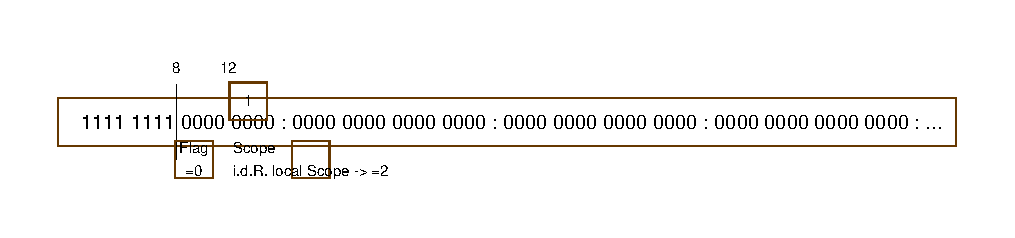
\includegraphics{multicast.pdf}
	\caption{Bit-Einteilung IPv6 Multicast Adresse}
\end{figure}

\textrightarrow\space \textbf{ff02:: /16}

\textbf{Beispiele:}
\begin{itemize}
    \item ff02::1 \textrightarrow\space All Nodes
    \item ff02::2 \textrightarrow\space All Routers
\end{itemize}


\subsubsection{Neighbor Discovery Protocol (NDP)}

Idee: 2-Schrittverfahren um 'etwas' über das Netz zu erfahren
\begin{enumerate}
    \item Host sendet eine 'Solicitation' (= Aufforderung)
    \item Alle Betroffenen antworten mit einem 'Advertisement' (=Werbung/Anzeige)
\end{enumerate}

Beispiel:
\begin{enumerate}
    \item Host sendet Router Solicitation (=Multicast FF02::2)
    \item Alle Router antworten mit Router Advertisement
\end{enumerate}

\subsubsection{Stateless Address Auto Configuration (SLAAC)}

Prozess um ohne DHCP eine gültige Globale Adresse bekommen.\\
Ablauf:
\begin{enumerate}
    \item Host: RS (Router Solicitation)
    \item Alle Router: RA (Router Advertisement)\\
        \textrightarrow\space Host 'schneidet' vordere 64 Bit von Router IP ab und setzt sie mit seiner Interface ID zusammen
    \item Neue IP wird über DAD (Duplicate Address Detection)\\
    \textrightarrow\space Host hat eine Globale IP!
\end{enumerate}


\subsubsection{DHCPv6}

Weil bei SLAAC die DNS-Option fehlt, brauchen die Hosts aber die DNS-IP!

\textrightarrow\space DHCP Konfigurieren
\begin{itemize}
    \item Stateless DHCP : NDP (zusätzlich Optionen)
    \item Stateful DHCP  : Klassisch
        \begin{enumerate}
            \item Solicitation
            \item Advertisement
            \item (Request)
            \item (Acknowledge)
        \end{enumerate}
\end{itemize}

\subsection{Domain Name System (DNS)}

\subsubsection{Wichtige Begriffe}

\begin{itemize}
    \item FQDN: Fully qualified domain name
    \item WINS: Windows internet name server
    \item NetBIOS: Network basic input/output system
\end{itemize}

\subsubsection{Aufbau FQDN}

\begin{table}[H]
    \centering
    \begin{tabular}{|l|l|l|l|}
         \hline
         www.&tagesschau&.com&.\\\hline
         Host&Second Level Domain& First Level Domain & Root (Wurzel)\\\hline
    \end{tabular}
\end{table}

\textbf{Jede FQDN ist weltweit eindeutig!}

\subsubsection{NetBios Name Auflösung Reihenfolge}
\textbf{Bei H-Knoten:}
\begin{enumerate}
        \item Cache wird überprüft (Cache anzeigen: 'ipconfig -displaydns', Cache lösche: 'ipconfig -flushdns)
	\item Hosts/LMHosts Datei
	\item WINS (über DHCP Option)
        \item Broadcast
\end{enumerate}

\subsubsection{FQDN Auflösung}

\begin{figure}[H]
	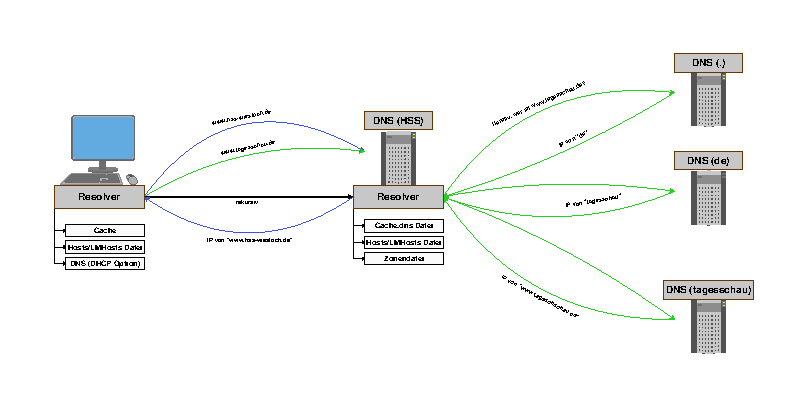
\includegraphics[width=\textwidth]{fqdn.pdf}
	\caption{Ablauf Auflösung FQDN}
\end{figure}


\subsubsection{Zonendatei}

hss-wiesloch.de.dns Datei in win32:\\
Record:

\begin{tabular}{|c|c|c|c|c|}
\hline
    \(<\)Name\(>\)&\(<\)TTL\(>\)&\(<\)Class\(>\)&\(<\)Type\(>\)&\(<\)Data\(>\)\\\hline
    www&Zeit in ms&IN&A&IPv4\\\hline
    www&Zeit in ms&IN&AAAA&IPv6\\\hline
\end{tabular}


\textbf{Name der Zonendatei:}
z.B.: www.hss-wiesloch.de = FQDN
\textrightarrow\space DNS \textrightarrow\space Datei: hss-wiesloch.de.dns



\textbf{Typen}:
\begin{itemize}
    \item MX: (Mail)IP v. Mail-Server
    \item SRV: (Service) z.B.: AD-Server
    \item CNAME: Alias (\(<\)name\(>\): lalala \(<\)type\(>\): CNAME \(<\)Data\(>\): www     =\textrightarrow\space lalala.hss-wiesloch.de ist alias für www.hss-wiesloch.de)
    \item NS: Name Server (\(<\)data\(>\): IP v. DNS)
    \item SOA: Start of authority \textrightarrow\space \(<\)data\(>\) enthält den primären DNS
    \item PTR: (PTR = Pointer)\\
    	www.hss-wiesloch.de  zu IP \textrightarrow\space forward lookup\\
    	10.1.2.3 zu name \textrightarrow\space reverse lookup\\
    	\textbf{Inverse}: 3.2.1.10\\
    Name Reverse Zone:\\
    	2.1.10.in-addr.dns\\
    	\begin{tabular}{|c|c|c|c|c|}
                \hline
                \(<\)Name\(>\)&\(<\)TTL\(>\)&\(<\)Class\(>\)&\(<\)Type\(>\)&\(<\)Data\(>\)\\\hline
                3&…&IN&PTR&FQDN: www.hss-wiesloch.de\\\hline
            \end{tabular}
\end{itemize}


\subsubsection{Exkurs: (Datensicherheit) / Ausfallsicherheit}

\textrightarrow\space Redundanz d.h. Datenbank existiert doppelt, dreifach…

\textrightarrow\space Replikation
\begin{enumerate}
    \item Kopie: Master \textrightarrow\space Slave(schreibgeschützt)
	             Primäre Zone \textrightarrow\space Sekundäre Zone
    \item Nur Änderungen: inkrementeller Zonentransfer
Jeder Server: Multimaster-Replikation (z.B. AD)
\end{enumerate}


\subsection{Dynamic Host Configuration Protokoll (DHCP)}

DHCP ermöglicht eine automatische Konfiguration von neu ins Netz eingebundenen Geräten.\\
Dabei werden folgende Einstellungen am Gerät konfiguriert:

\begin{itemize}
    \item Eigene IP-Adresse
    \item Netzmaske / Subnetzmaske
    \item Gateway
    \item DNS
    \item Time- und NTP-Server
\end{itemize}

Ohne DHCP müsste ein Administrator diese Einstellungen für jedes Gerät per Hand vornehmen.

\subsubsection{DHCP Server}
Der DHCP-Server ist ein Hintergrundprozess und wartet auf dem UDP-Port 67 auf die Anfrage eines DHCP-Clients, der sich mit dem Netzwerk verbinden möchte.\\
In einer vorher definierten Konfigurationsdatei befinden sich die erforderlichen Parameter, die dann automatisch zum Client gesendet werden, um diesen zu konfigurieren.

Es gibt drei unterschiedliche Betriebsmodi eines DHCP-Servers:

\begin{enumerate}
    \item \textbf{Manuelle Zuordnung: }Auch als statistisches DHCP bezeichnet. Die am DHCP-Server festgelegten IP-Adressen werden festen MAC-Adressen (der Hardware-Adresse des einzelnen Netzwerkadapters - zur eindeutigen Identifikation des Gerätes) zugeordnet. Die Adressen werden fest vergeben und es ergibt sich der Nachteil, dass keine zusätzlichen Clients in das Netz eingebunden werden können, da die Adressen nur fest vergeben werden. Aus Sicherheitsperspektive kann das aber auch erwünscht sein.
    \item \textbf{Automatische Zuordnung:} Bei dieser Zuordnung wird ein festgelegter Bereich von IP-Adressen durch den DHCP-Server zugeordnet. Sobald die Adressen miteinander verknüpft sind, bleiben auch diese auf unbestimmte Zeit verbunden. Der Nachteil ist, dass neue Clients keine IP-Adresse erhalten, wenn der Bereich komplett vergeben ist.
    \item \textbf{Dynamische Zuordnung:} Im Unterschied zu den beiden vorherigen Verfahren ist bei der dynamischen Zuordnung die Zuordnung zeitlich begrenzt. Heißt, dass der DHCP-Server innerhalb seiner Konfigurationsdatei festlegt, wie lange eine IP-Adresse an einen Client gegeben werden darf. Diese vom Administrator festgelegte Zeit wird in der IT auch als "Lease-Time" (dt. Leihdauer) bezeichnet.
\end{enumerate}



\end{document}